\documentclass[14pt,a4paper]{extarticle}
\usepackage[T2A]{fontenc}
\usepackage[utf8]{inputenc}
\usepackage[english,russian]{babel}
\usepackage{lmodern}
\usepackage{geometry}
\usepackage{array}
\usepackage{tabularx}
\usepackage{longtable}
\usepackage{ltablex}
\usepackage{booktabs}
\usepackage{hyperref}
\usepackage{indentfirst}
\usepackage{microtype}
\usepackage{graphicx}
\usepackage{setspace}
\usepackage{listings}
\usepackage{graphicx}
\usepackage{caption}
\usepackage{float}
\usepackage{tocloft}
\usepackage{titlesec}
\usepackage{newtxtext,newtxmath}

\titleformat{\section}        % форматируем \section
  {\normalfont\bfseries}      % стиль: обычный + жирный
  {\thesection.}              % номер секции с точкой
  {2mm}                       % расстояние между номером и текстом
  {}                           % перед заголовком можно добавить что-то
\titlespacing*{\section}{1.5cm}{*3}{*1}  % {отступ слева}{отступ сверху}{отступ снизу}

\captionsetup{justification=centering}
\renewcommand{\ttdefault}{cmtt}
\keepXColumns
\setlength{\parindent}{3em}
\newgeometry{left=2.5cm,right=2.5cm,top=3cm,bottom=2.5cm}

\renewcommand{\contentsname}{\hspace*{4em}{\smallСодержание}}
\setlength{\cftbeforesecskip}{0.5em}
\renewcommand{\cftsecleader}{\cftdotfill{\cftdotsep}}
\renewcommand{\cftsecaftersnum}{.\hspace{2mm}}

\title{Отчёт по "Программно-аппаратные средства интеллектуальных систем"}
\author{Выполнил студент группы М-РИТ-25-1, Станиславчук Сергей}

\begin{document}

\setstretch{1.5}
\noindent
\begin{minipage}[t]{0.01\textwidth}
    \includegraphics{~/programmer/++Programmer/5_1/LSTU.jpg}
\end{minipage}%
\begin{minipage}[c]{1.1\linewidth}
    \centering
    {\small
    МИНИСТЕРСТВО НАУКИ И ВЫСШЕГО ОБРАЗОВАНИЯ РФ \\[1em]
    ФЕДЕРАЛЬНОЕ ГОСУДАРСТВЕННОЕ БЮДЖЕТНОЕ \\
    ОБРАЗОВАТЕЛЬНОЕ УЧРЕЖДЕНИЕ ВЫСШЕГО ОБРАЗОВАНИЯ \\
    «ЛИПЕЦКИЙ ГОСУДАРСТВЕННЫЙ ТЕХНИЧЕСКИЙ УНИВЕРСИТЕТ»
    }
\end{minipage}%

\vspace{3em}

\noindent
\hspace{1em}%
\begin{minipage}[t]{0.8\textwidth}
\textbf{Институт} \hspace{2em} компьютерных наук \\
\textbf{Кафедра} \hspace{2em} автоматизированных систем управления
\end{minipage}


\vspace{6em}

\begin{center}
\textbf{ПРАКТИЧЕСКАЯ РАБОТА №3} \\
по дисциплине \\ <<Программно-аппаратные средства интеллектуальных систем>>
\end{center}

\vspace{6em}

\noindent
\begin{tabular*}{\textwidth}{@{\extracolsep{\fill}} l c r }
    Студент М-РИТ-25-1 & \makebox[4cm]{\hrulefill} & Станиславчук С.М. \\[2em]
Руководитель & \\
Ст. преподаватель & \makebox[4cm]{\hrulefill} & Болдырихин О.В. \\
\end{tabular*}

\vfill
\begin{center}
    Липецк, 2025
\end{center}

\thispagestyle{empty}

\newpage
\tableofcontents
\newpage

\section{Задание, конкретизированное вариантом}
\begin{sloppypar}
Цель работы - исследование взаимозависимости между технико-эксплуатационными
    показателями супекомпьютерных систем.

    Построить диаграму рассеяния (точечную диаграмму, scatter plot) и
    рассчитать коэффициент корреляции двух заданных показателей (табл. 3.1) для
    двух рейтингов. Оценить разницу результатов для этих рейтингов. Оценить
    наличие и характер взаимосвязи между показателями.
\end{sloppypar}

Вариант 17 -> 2\&7:

2. Реальная производительность по HPL: Rmax
\newline7. Эффективность архитектуры по HPL: Rmax/Rpeak


\newpage
\section{Описание исследуемых показателей}
Rmax - наивысший результат, полученный при использовании системы тестов Linpack
(реализация HPL). Это число используется для сравнения быстродействия
компьютеров. Измеряется в GFLOPS.

Rpeak - теоретический максимум производительности. Определяется путем умножения
количества единиц измерения с плавающей запятой на процессор, умноженное на
количество команд с плавающей запятой, которые могут быть выполнены в секунду.
Измеряется в GFLOPS

Отношение HPL Efficiency = Rmax / Rpeak характеризует архитектурную
сбалансированность системы. Это соотношение можно рассматривать как коэффициент
эффективности, хотя использование этого результата для определения ценности
систем может оказаться непродуктивным. 75\% от 1000 - это то же самое, что и
100\% от 750, и если у них одинаковые денежные затраты и затраты на
электроэнергию, то разницы нет.

\sloppy

\section{Исходные данные}

Для анализа, в качестве исходных данных, были выбраны следующие рейтинги для
сравнения: 1993.06 и 2009.06.

\section{Использованные программные средства}
Для выполнения анализа использовался язык программирования Python 3.
Необходимые библиотеки устанавливались с помощью команды:

\begin{sloppypar}
\texttt {pip install requests lxml mapplotlib pandas numpy scipy tabulate}
\end{sloppypar}

\begin{sloppypar}
С помощью библиотеки \texttt{requests} выполнялось автоматическое скачивание XML-файлов с сайта \texttt{top500.org}

Модуль «\texttt{lxml.etree}» применялся для разбора структуры XML.
Из каждого документа (рейтинга) извлекается значение <<\texttt{Rmax}>> и <<\texttt{Rpeak}>>
с помощью функции \texttt{findtext}, затем в каждой извлечённой строке
рассчитывается показатель «\texttt{HPL Efficiency }» по следующей формуле:
\texttt{ eff = rmax / rpeak }. Полученные записи rmax, rpeak, eff, а также list\_id добавляются в общий массив пользовательской
структуры для последующей обработки.

Далее в функции \texttt{ scatter } рассчитывается коэффициент корреляции Пирсона между \texttt{Rpeak} и \texttt{HPL Efficiency} с помощью
функции из модуля \texttt{numpy} <<\texttt{corrcoef}>>.

Результаты записываются в единую таблицу (DataFrame) с помощью библиотеки \texttt{pandas}.

Исходя из полученной таблицы, строятся две диаграммы рассеяния (scatter plot),
а поверх нее сплошным текстом указываются показатели коэффициента Пирсона для
рейтингов 1993.06 и 2009.06 соответственно.
\end{sloppypar}

По оси X - HPL Rmax.
\newlineПо оси Y - HPL Efficiency.

Текст программы представлен в приложении 1.

\newpage
\section{Ход и результаты исследования: построение диаграмм рассеяния, расчёт
коэффициентов корреляции.}
    Полученная диаграмма рассеяния для рейтинга TOP500 1993.06, между двумя
    показателями: HPL Efficiency и HPL Rmax, представлена на рисунке 1.

\begin{figure}[H]
    \label{fig:pic1}
    \centering
    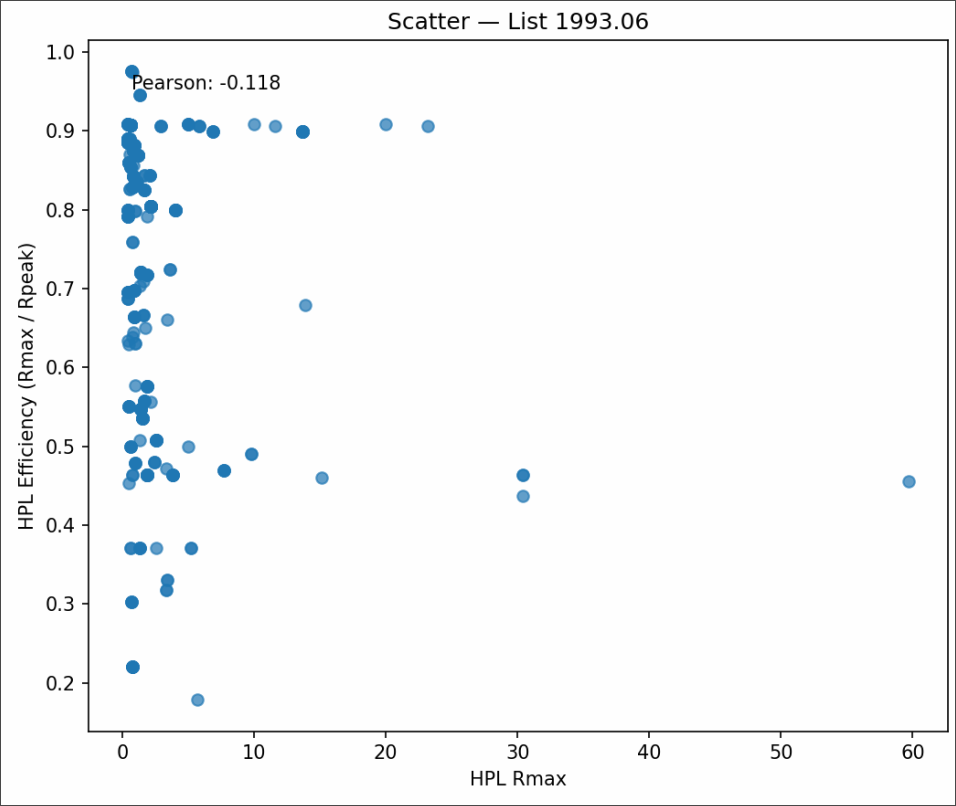
\includegraphics[width=0.78\textwidth]{pic1.png}
    \refstepcounter{figure}
    \caption*{Рисунок \thefigure\ — Диаграмма рассеяния 1993.06}
\end{figure}

    Полученная диаграмма рассеяния для рейтинга TOP500 2009.06, между двумя
    показателями: HPL Efficiency и HPL Rmax, представлена на рисунке 2.


\begin{figure}[H]
    \label{fig:pic2}
    \centering
    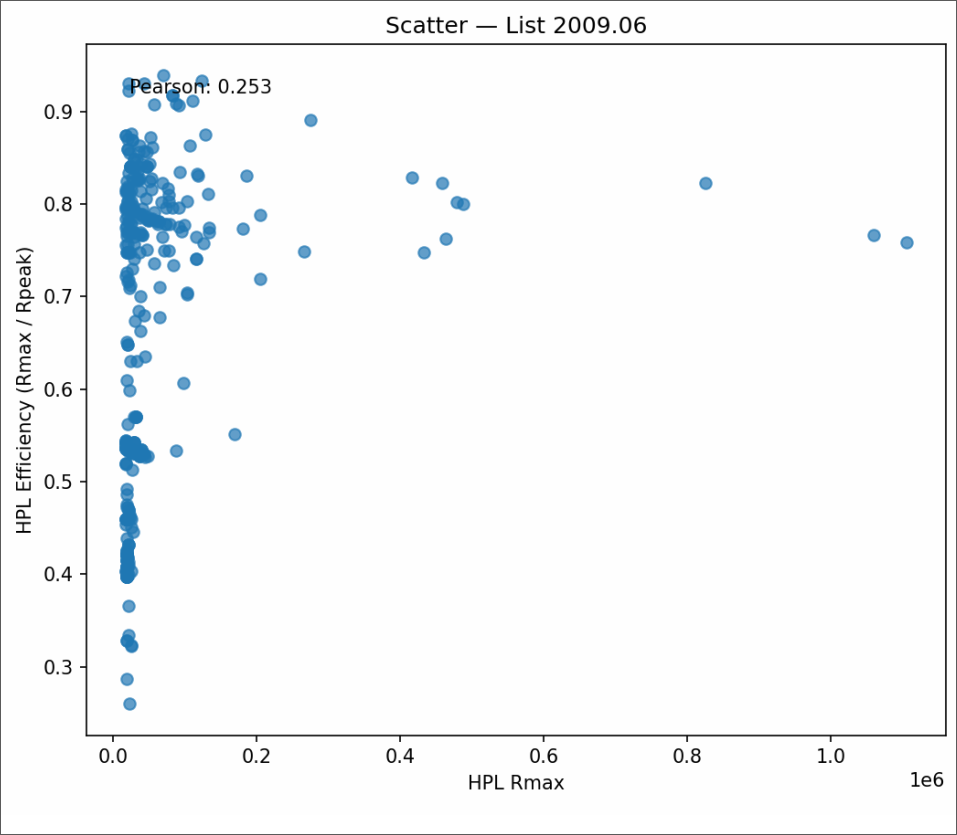
\includegraphics[width=0.78\textwidth]{pic2.png}
    \refstepcounter{figure}
    \caption*{Рисунок \thefigure\ — Диаграмма рассеяния 2009.06}
\end{figure}

Полученные коээфициенты корреляции Пирсона: -0.118 и 0.253 для рейтингов
1993.06 и 2009.06 соответственно

\section{Выводы}
1993.06. Диаграмма показывает полное отсутствие связи между HPL Rmax и
архитектурной эффективностью. Корреляция отрицательная и близка к нулю
(–0.118). Точки разбросаны хаотично: даже системы с очень низким Rmax могут
иметь высокую эффективность, и наоборот — мощные машины демонстрируют низкие
коэффициенты Rmax/Rpeak. Это объясняется тем, что ландшафт HPC в начале 1990-х
был крайне разнородным: векторные ЭВМ, SMP-сервера и экспериментальные
суперкомпьютеры использовали разные архитектурные подходы, несовместимые
методики расчёта Rpeak, и в целом не обеспечивали стабильного масштабирования
LINPACK при росте числа узлов. Отсюда — отсутствие какой-либо зависимости между
производительностью и эффективностью.

2009.06 На диаграмме уже видна слабая положительная связь между показателями:
более мощные системы чаще демонстрируют более высокую эффективность HPL.
Корреляция +0.253 хоть и небольшая, но это заметный контраст с 1993 годом.
Облако точек становится более плотным: большинство машин имеют эффективностьМ
0.75–0.9, а экстремальные значения почти исчезают. Это следствие перехода
отрасли к зрелым кластерным архитектурам, стандартизированным CPU,
распространению InfiniBand в качестве высокоскоростной сети и унификации
программного стека MPI. Системы проектируются сбалансированно, и их масштаб уже
напрямую влияет на способность эффективно выполнять LINPACK.

Между периодами виден качественный скачок развития HPC. В 1993
производительность суперкомпьютера не имела никакой связи с его архитектурной
эффективностью: каждая машина была индивидуальным инженерным экспериментом. В
2009, напротив, прослеживается тенденция, что более крупные и мощные системы
демонстрируют более высокую эффективность — отрасль пришла к стандартным
решениям и оптимизированным кластерным архитектурам. Иными словами, если в 1993
эффективность диктовалась исключительно особенностями конкретной машины и часто
была случайна, то в 2009 она становится системным свойством, растущим вместе с
масштабом и качеством архитектуры.

\newpage
\section*{Приложение 1. Код программы}
\begin{verbatim}

#!/usr/bin/env python3
"""
Variant #17
Correlation:
    X = HPL Rmax
    Y = HPL Efficiency = Rmax / Rpeak

For lists:
    1 → 1993.6
    2 → 2007.06
"""

import os
import numpy as np
import pandas as pd
import matplotlib.pyplot as plt
from lxml import etree
from tabulate import tabulate

XML_DIR = "xml"

LISTS = {
    1: (1993, 6),
    2: (2009, 6),
}

OUT_PLOT = "variant17_scatter.png"


def load_xml(year, month):
    fname = f"TOP500_{year}{month:02d}.xml"
    path = os.path.join(XML_DIR, fname)
    if not os.path.exists(path):
        print(f"[ERR] missing XML file: {path}")
        return None
    with open(path, "rb") as f:
        return etree.fromstring(f.read())


def parse_list(root, list_id):
    ns = {"top500": root.nsmap.get("top500")}

    rows = []
    for site in root.findall("top500:site", namespaces=ns):
        try:
            rmax = float(site.findtext("top500:r-max", namespaces=ns))
            rpeak = float(site.findtext("top500:r-peak", namespaces=ns))

            if rmax <= 0 or rpeak <= 0:
                continue

            eff = rmax / rpeak

            rows.append({
                "list": list_id,
                "rmax": rmax,
                "rpeak": rpeak,
                "eff_hpl": eff
            })
        except:
            continue

    return rows


def scatter(df, label, ax):
    x = df["rmax"]
    y = df["eff_hpl"]

    ax.scatter(x, y, alpha=0.7)
    ax.set_xlabel("HPL Rmax")
    ax.set_ylabel("HPL Efficiency (Rmax / Rpeak)")
    ax.set_title(f"Scatter — {label}")

    corr = np.corrcoef(x, y)[0, 1]
    ax.text(0.05, 0.95, f"Pearson: {corr:.3f}", transform=ax.transAxes, va="top")

    return corr


def main():
    all_rows = []

    for list_id, (yy, mm) in LISTS.items():
        root = load_xml(yy, mm)
        if root is None:
            continue
        rows = parse_list(root, list_id)
        print(f"[OK] List {list_id} parsed: {len(rows)} rows")
        all_rows.extend(rows)

    df = pd.DataFrame(all_rows)

    print("\n=== Parsed data ===")
    print(tabulate(df.head(10), headers="keys", tablefmt="github", floatfmt=".3f"))

    df32 = df[df["list"] == 1]
    df33 = df[df["list"] == 2]

    fig, (ax1, ax2) = plt.subplots(1, 2, figsize=(14, 6))

    c32 = scatter(df32, "List 1993.06", ax1)
    c33 = scatter(df33, "List 2009.06", ax2)

    plt.tight_layout()
    plt.savefig(OUT_PLOT, dpi=150)
    plt.close()

    print(f"\n[PLOT] saved as {OUT_PLOT}")

    print("\n=== Correlations ===")
    print(f"1993.06: {c32:.4f}")
    print(f"2009.06: {c33:.4f}")


if __name__ == "__main__":
    main()


\end{verbatim}

\end{document}
